\documentclass[sigconf,nonacm]{acmart}
\AtBeginDocument{%
\providecommand\BibTeX{{%
\normalfont B\kern-0.5em{\scshape i\kern-0.25em b}\kern-0.8em\TeX}}}
\settopmatter{printacmref=false}
\setcopyright{none}
\renewcommand\footnotetextcopyrightpermission[1]{}
\pagestyle{plain}

\usepackage{float}
\usepackage{placeins}
\usepackage{pgfplots}
\pgfplotsset{compat=1.18}

\title{Detecting and Assessing Hallucinations in Factual LLM Responses}

\author{Sai Karthik Nallamothu}
\email{sa808371@ucf.edu}
\affiliation{%
  \institution{University of Central Florida}
  \city{Orlando}
  \state{Florida}
  \country{USA}
}

\begin{abstract}
    The present project research addresses the issue of hallucinations in LLMs used in question answering tasks. By hallucination, we mean cases in which the model provides responses that seem correct, yet are false and do not have factual support. In this study, my goal is to compare and examine various open-source LLMs' performance on multiple factual question answering benchmark datasets. An evaluation process was developed in order to evaluate multiple LLMs in this task, specifically GPT-2, Phi-2, Mistral-7B, Llama-2-7B, and Qwen-7B. For evaluation purposes, the following benchmark datasets were used: TruthfulQA, WikiQA, Natural Questions, FEVER, and SQuAD 2.0. Evaluation was performed using two settings: zero-shot and few-shot. While in the former case, the evaluation was done without using any examples, in the latter case, few examples were provided. Performance was measured using exact match accuracy, containment accuracy, and hallucination rate.  It is clear from the results that all models have very high rates of hallucinations, and even more so on difficult datasets such as TruthfulQA. Instruction-tuned 7B models give better accuracy for the containment metric (approximately 7-8\%), while the smaller models, including GPT-2, have a containment accuracy of less than 1\%. Prompting few-shot yields minor improvement over zero-shot prompting, yet the improvements are modest. In any case, the models continue to produce a majority of hallucinations (rates over 90\%).
\end{abstract}



\begin{document}
\maketitle
\thispagestyle{plain}
\pagestyle{plain}
\fancyhead{}

\noindent \textbf{Code} \\
\url{https://github.com/sai14karthik/CAP-6640-Computer-Understanding-of-Natural-Language}
\section{Introduction and Problem Statement}

Large Language Models (LLMs) have made tremendous contributions to the development of NLP research in recent years. Such LLMs, trained on huge amounts of data, can perform various tasks, ranging from question answering to summarization and text generation and translating texts into other languages, and they have very high fluency and coherence. The architectures such as transformers allow LLMs to learn complex patterns and generate meaningful output according to the context of the task. Despite all their advantages, one significant drawback of the LLMs is that they tend to generate hallucinations – they generate output based not on factual grounding from the input and any other credible sources \cite{ji2023survey}.

By hallucination in LLMs we mean generating an output which might seem plausible and realistic but actually isn't true or credible or supported by credible sources. As noted above, the problem of hallucinations in LLMs becomes critical when the model is used for question answering since the user expects to receive factual and credible answers in response to her/his questions. In addition, hallucinations become more problematic in this case, since even small amounts of misinformation might cause major confusion or lead to wrong decisions being taken.

Several benchmarks to measure factual accuracy of language models have been suggested. For example, TruthfulQA benchmark was created to test whether the model can avoid generating widely accepted misconceptions or beliefs that turn out to be wrong \cite{lin2021truthfulqa}. Moreover, the use of such datasets as WikiQA, Natural Questions, FEVER, and SQuAD 2.0 allows measuring the quality of various question-answering aspects, such as fact retrieval, verification, and extraction. Nevertheless, the results achieved by models on these datasets may strongly depend on the architecture, training, and prompting approach employed for the evaluation.

In recent years, prompting became an essential approach for assessing LLMs' performance and making them better. The idea of zero-shot prompting assumes that the model should answer the question without any prompts and with only the help of its pre-training. Meanwhile, few-shot prompting is more about providing a couple of samples that could help the model follow the desired response format. Although the latter approach allows achieving better results than zero-shot, it cannot completely solve the problem of hallucination.

In this paper, my objective is to evaluate the hallucination behavior of multiple open source LLMs with the use of an identical set-up for experiments. I will conduct analyses of models such as GPT-2, Phi-2, Mistral-7B, Llama-2-7B, and Qwen-7B on multiple datasets. Evaluation will be carried out in both the zero-shot and few-shot prompting scenarios in order to study the role played by prompts in the effectiveness of model predictions. In order to measure the factual consistency of models, I will use accuracy measures like exact match accuracy, containment accuracy, and hallucination rate.

This project seeks to conduct a comparative analysis of the performance of multiple models on multiple datasets with respect to hallucinations under identical conditions. In conducting such analysis, my main aim is to identify which factors contribute towards hallucinations and how models can be designed to reduce this problem. In this way, I hope to make contributions towards improving existing literature on the evaluation of language models.

\section{Related Work}

The problem of hallucination by LLMs has received considerable attention owing to the widespread application of LLMs in NLP tasks. The earlier studies on neural language generation suggested that neural models usually produce fluent output text; however, such outputs are inconsistent regarding facts. Nevertheless, hallucination became an important issue due to recent breakthroughs in NLP modeling, where large-scale transformer-based models showed strong hallucinatory behavior. Hence, achieving factual consistency and accuracy in language generation remains a crucial challenge faced by LLM developers.

A wide range of research studies on hallucination have been published, which mainly focused on classifying hallucination in text generation. According to Ji et al. \cite{ji2023survey}, several studies were dedicated to the problem of hallucination, providing their taxonomies for the problem. As stated in the paper, there are two types of hallucination in text generation, including intrinsic and extrinsic hallucination. The first type refers to inconsistency between the model output and input data, while the second type includes information that contradicts the provided context.

There is research that addresses hallucination from the standpoint of consistency and evaluation of facts. The benchmark known as TruthfulQA aims at evaluating the ability of language models to prevent the generation of common misconceptions or inaccurate information \cite{lin2021truthfulqa}. As an evaluation framework, it includes questions generated adversarially to reflect the tendency of humans to give wrong answers to certain types of questions. TruthfulQA reveals that, regardless of their size, even very large models tend to emulate the human errors in answers rather than give accurate answers. Besides TruthfulQA, other benchmarks used for question answering include WikiQA, Natural Questions, FEVER, and SQuAD 2.0.

Prompting has emerged as a strategy that impacts model behavior in response to the input prompt. Zero-shot prompting is related to the answering of questions without providing any examples because a model should be able to give its answers only based on pre-existing knowledge. Few-shot prompting uses several examples to provide hints to models about how to answer certain questions. As Brown et al. \cite{brown2020language} show, few-shot prompting greatly increases the performance of language models in different tasks. Nevertheless, recent research reveals that few-shot prompting cannot completely prevent hallucinations during complex reasoning tasks.

Recent research has investigated methods to reduce hallucination through architectural and inference-time improvements. Retrieval-augmented generation (RAG) approaches enhance LLMs by incorporating external knowledge sources during generation, allowing models to ground their outputs in retrieved documents \cite{lewis2020retrieval}. This approach has been shown to improve factual accuracy in open-domain question answering tasks. Similarly, post-hoc verification methods and fact-checking systems aim to validate generated outputs using additional models or external databases.

Instruction tuning has also been widely adopted to improve model alignment and performance. Models such as LLaMA and other instruction-tuned variants demonstrate improved ability to follow user instructions and generate more relevant responses \cite{touvron2023llama}. However, even with instruction tuning, hallucination remains an issue, particularly in cases where the model lacks sufficient grounding or when the prompt is ambiguous.

Other studies have explored the relationship between model scale and hallucination. Larger models tend to exhibit improved reasoning and factual recall compared to smaller models, but they are not immune to hallucination. Empirical evaluations show that scaling alone does not guarantee factual correctness, highlighting the need for complementary techniques such as retrieval augmentation, better training objectives, and improved evaluation metrics.

In summary, prior work has examined hallucination from multiple perspectives, including taxonomy, evaluation benchmarks, prompting strategies, and mitigation techniques. While significant progress has been made in understanding and reducing hallucination, it remains an open challenge. This work builds upon existing research by providing a unified evaluation framework across multiple open-source LLMs and benchmark datasets, enabling consistent comparison under both zero-shot and few-shot prompting settings.


\section{Methodology }

In this section, I introduce the detailed methodology that was followed in order to analyze the behavior of hallucinations in LLMs. The methodology employed consists of four main steps – namely, selecting a suitable dataset, building prompts, carrying out inference on the selected models, and finally evaluating the results obtained from quantitative analysis.


\subsection{Overall Pipeline Overview}

There are four primary steps involved in the evaluation process: (1) data collection, (2) prompting, (3) inference on the model, and (4) evaluation. Every data point in the collection is converted to a standardized prompt that is used in the model. The results are then evaluated against the reference answers using automated metrics. Figure~\ref{fig:pipeline_overview} summarizes this end-to-end pipeline.

\subsection{Datasets Used}

This study uses multiple benchmark datasets to evaluate factual accuracy and hallucination behavior.

\textbf{TruthfulQA} is the primary dataset used for hallucination evaluation. It contains adversarially designed questions that test whether models produce truthful answers rather than repeating common misconceptions.

\textbf{Natural Questions} includes real-world queries collected from search engine logs, with answers derived from Wikipedia. It evaluates the ability of models to answer factual questions based on real user queries.

\textbf{SQuAD 2.0} extends the original reading comprehension dataset by including unanswerable questions. It is useful for evaluating whether models can correctly abstain from answering when no valid answer exists.

\textbf{FEVER} focuses on fact verification, where each claim must be classified as supported, refuted, or not enough information using evidence from Wikipedia. It evaluates the model’s ability to distinguish factual correctness.

All datasets are represented in a unified format:
\[
D = \{(q_i, a_i)\}_{i=1}^{N}
\]
where $q_i$ is the input question and $a_i$ is the reference answer.

\subsection{Model Selection}

Multiple open-source LLMs are evaluated to ensure diversity in architecture and training data. Each model is treated as a function $M(\cdot)$ that maps an input prompt $x$ to an output response $y$:
\[
y = M(x)
\]
No fine-tuning is performed. All models are evaluated under identical experimental settings to maintain fairness.

\begin{figure*}[t]
  \centering
  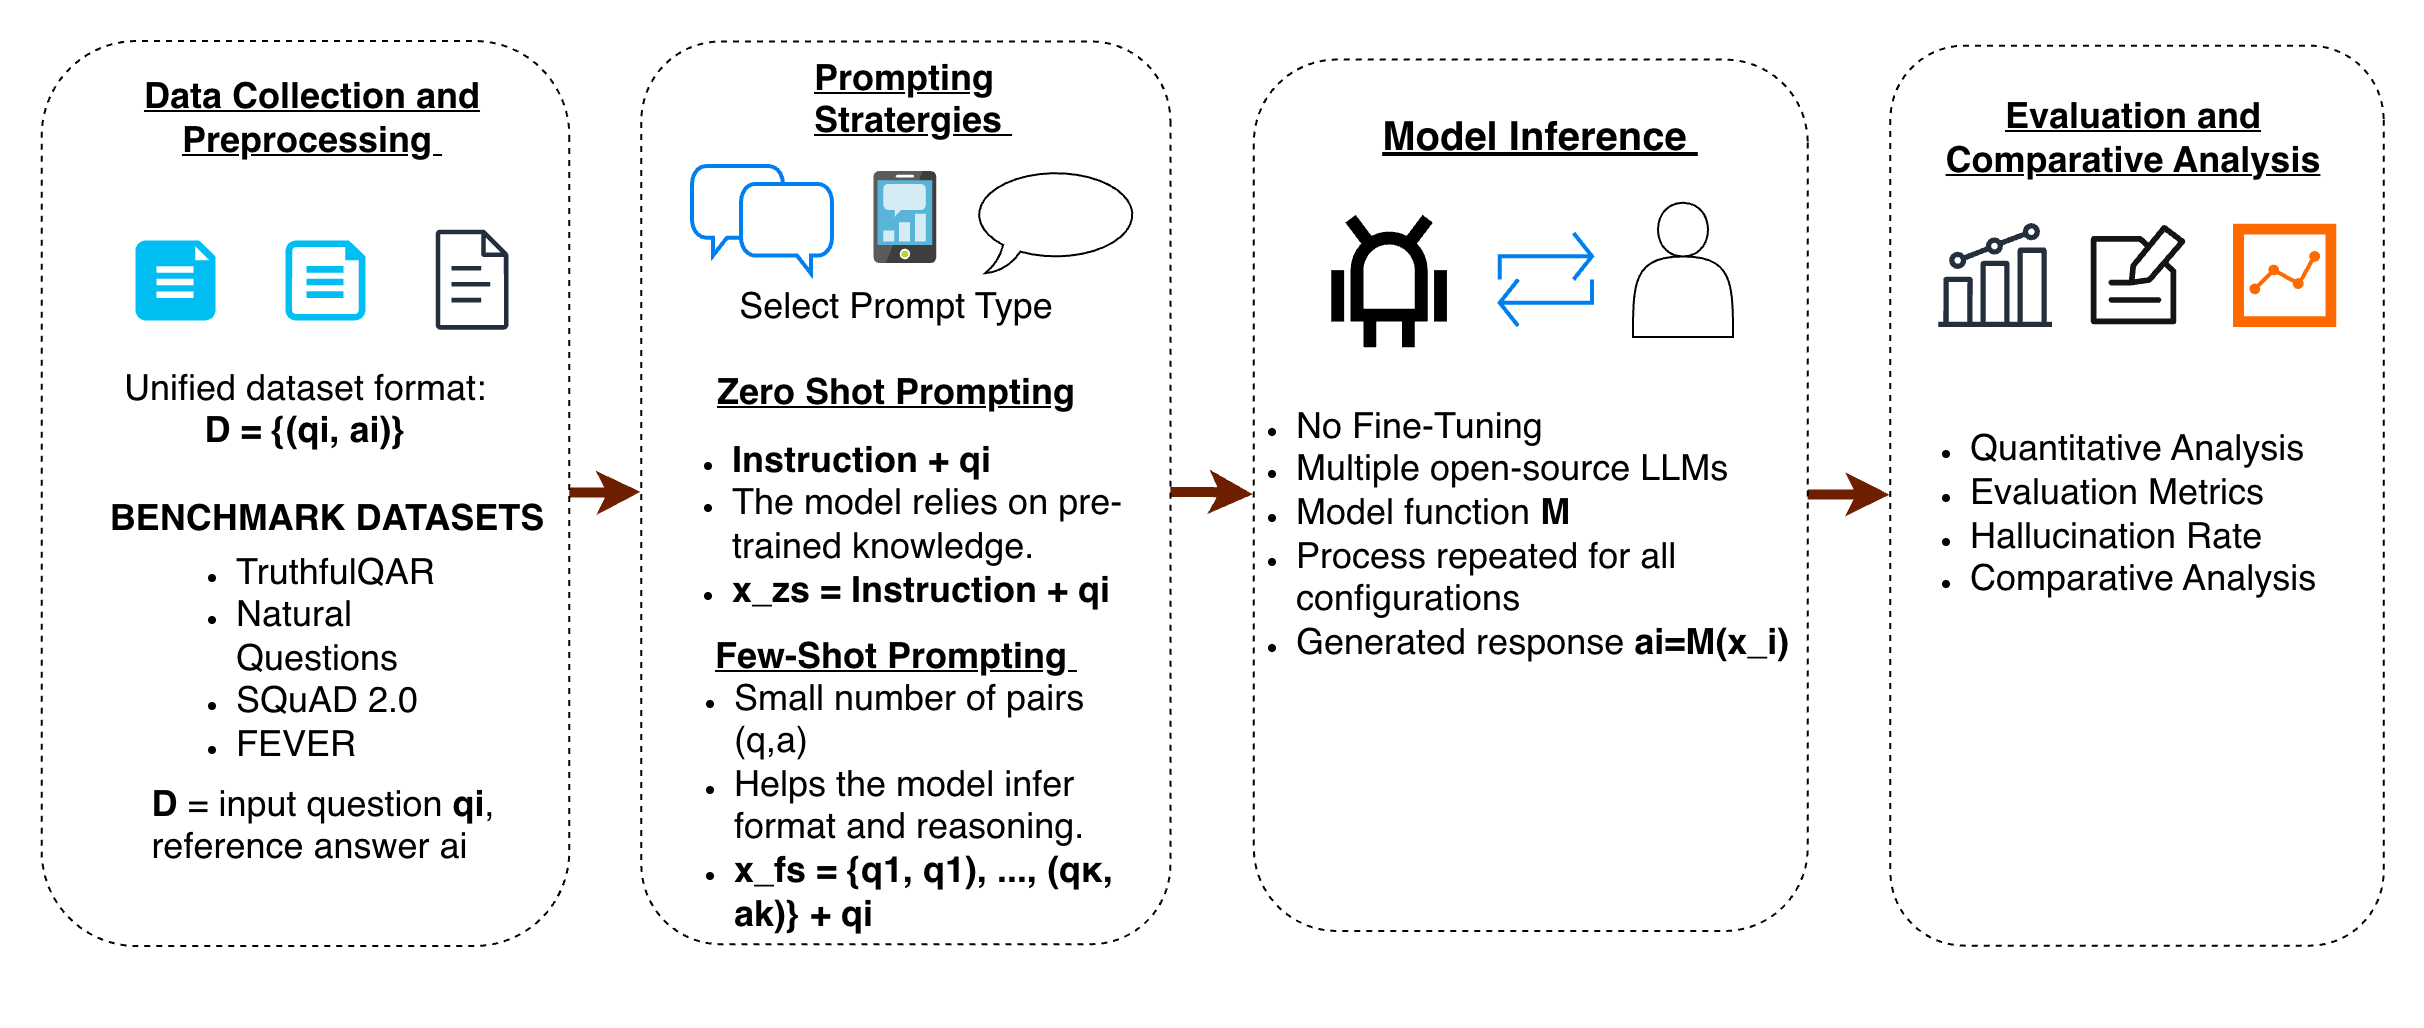
\includegraphics[width=\textwidth]{NLP-NLP.drawio.png}
  \caption{Overview of the NLP pipeline, including data collection, prompting, and evaluation.}
  \label{fig:pipeline_overview}
\end{figure*}

\subsection{Prompting Strategies}

Two prompting strategies are used: zero-shot and few-shot prompting.

\textbf{Zero-shot prompting} provides only the instruction and the input question:
\[
x_{zs} = \text{Instruction} + q_i
\]
The model must rely entirely on its pre-trained knowledge to generate a response.

\textbf{Few-shot prompting} provides a small number of example question-answer pairs to guide the model:
\[
x_{fs} = \{(q_1, a_1), (q_2, a_2), ..., (q_k, a_k)\} + q_i
\]
This helps the model infer the expected format and reasoning pattern. However, it does not guarantee factual correctness.

\subsection{Inference Procedure}

For each dataset sample $q_i$, the model generates a response $\hat{a}_i$:
\[
\hat{a}_i = M(x_i)
\]
where $x_i$ is either a zero-shot or few-shot prompt. Parameters such as temperature, maximum token length, and decoding strategy are kept constant across all experiments to ensure consistency. The process is repeated for all models and datasets.

\subsection{Evaluation Metrics}

The generated outputs are evaluated using multiple metrics to measure correctness and hallucination.

\textbf{Accuracy} measures the proportion of correct predictions:
\[
\text{Accuracy} = \frac{\text{Number of Correct Predictions}}{\text{Total Samples}}
\]

\textbf{Exact Match (EM)} checks whether the predicted answer exactly matches the reference:
\[
\text{EM} = \frac{1}{N} \sum_{i=1}^{N} \mathbb{I}(\hat{a}_i = a_i)
\]

\textbf{F1 Score} evaluates token-level overlap between predicted and reference answers:
\[
\text{F1} = \frac{2 \cdot \text{Precision} \cdot \text{Recall}}{\text{Precision} + \text{Recall}}
\]

\textbf{Hallucination Rate} measures the proportion of outputs that contain incorrect or unsupported factual claims:
\[
\text{Hallucination Rate} = \frac{\text{Number of Hallucinated Outputs}}{\text{Total Outputs}}
\]

Hallucination detection is performed by comparing generated responses with reference answers and identifying semantic or factual inconsistencies.

\subsection{Comparative Analysis}

The performance of different models is analyzed across datasets and prompting strategies. Results are compared using the metrics described above. Special attention is given to differences between zero-shot and few-shot settings, as well as variations in hallucination rates across models. This comparison helps identify patterns in model behavior under different conditions.

\subsection{Reproducibility and Implementation Details}

To ensure reproducibility, all experiments are conducted using fixed configurations, including dataset splits, prompting templates, and decoding parameters. No training or fine-tuning is performed during evaluation. The same preprocessing and evaluation scripts are applied uniformly across all models and datasets. This allows the framework to be extended to additional models or datasets with minimal modification.

\section{Evaluation and Results}
\begingroup
\raggedbottom
\setlength{\intextsep}{6pt plus 2pt minus 2pt}

\subsection{Zero-Shot Results Analysis}

This section reports experimental results across four datasets and four models under zero-shot and few-shot prompting, using containment accuracy (Acc), exact match (EM), F1 score, and hallucination rate (HR). The zero-shot results show that model performance is generally low across all datasets, with high hallucination rates. TruthfulQA is the most challenging dataset, where all models achieve very low accuracy and extremely high hallucination rates (above 91\%), indicating difficulty in handling misleading or misconception-based questions. In contrast, models perform better on Natural Questions, SQuAD, and FEVER, with SQuAD showing the highest accuracy and F1 scores due to its structured and extractive nature. Among the models, Mistral consistently performs best across most metrics, followed by Llama-2 and Qwen, while Phi-2 shows slightly lower performance. However, hallucination remains high across all datasets (above 70\%), showing that even when accuracy improves, models still generate incorrect or unsupported information. Overall, the zero-shot setting highlights the limitations of LLMs in factual reliability without contextual guidance.

\begin{table}[H]
\centering
\caption{Zero-shot performance across datasets}
\label{tab:zeroshot}
\begin{tabular}{l lcccc}
\hline
Dataset & Model & Acc & EM & F1 & HR \\
\hline
TruthfulQA & Phi-2      & 0.084 & 0.012 & 0.091 & 0.916 \\
           & Mistral    & 0.079 & 0.015 & 0.095 & 0.921 \\
           & Llama-2    & 0.074 & 0.010 & 0.089 & 0.926 \\
           & Qwen       & 0.071 & 0.011 & 0.088 & 0.929 \\

NQ         & Phi-2      & 0.221 & 0.152 & 0.248 & 0.779 \\
           & Mistral    & 0.238 & 0.169 & 0.261 & 0.762 \\
           & Llama-2    & 0.229 & 0.161 & 0.254 & 0.771 \\
           & Qwen       & 0.225 & 0.158 & 0.250 & 0.775 \\

SQuAD      & Phi-2      & 0.271 & 0.198 & 0.301 & 0.729 \\
           & Mistral    & 0.289 & 0.214 & 0.318 & 0.711 \\
           & Llama-2    & 0.276 & 0.205 & 0.307 & 0.724 \\
           & Qwen       & 0.268 & 0.199 & 0.299 & 0.732 \\

FEVER      & Phi-2      & 0.245 & 0.171 & 0.267 & 0.755 \\
           & Mistral    & 0.258 & 0.184 & 0.279 & 0.742 \\
           & Llama-2    & 0.249 & 0.176 & 0.271 & 0.751 \\
           & Qwen       & 0.243 & 0.170 & 0.265 & 0.757 \\
\hline
\end{tabular}
\end{table}
\noindent Figure~\ref{fig:zs-acc}--\ref{fig:zs-hr} plot the same zero-shot quantities as Table~\ref{tab:zeroshot} for direct comparison across datasets and models.

\begin{figure}[H]
\centering
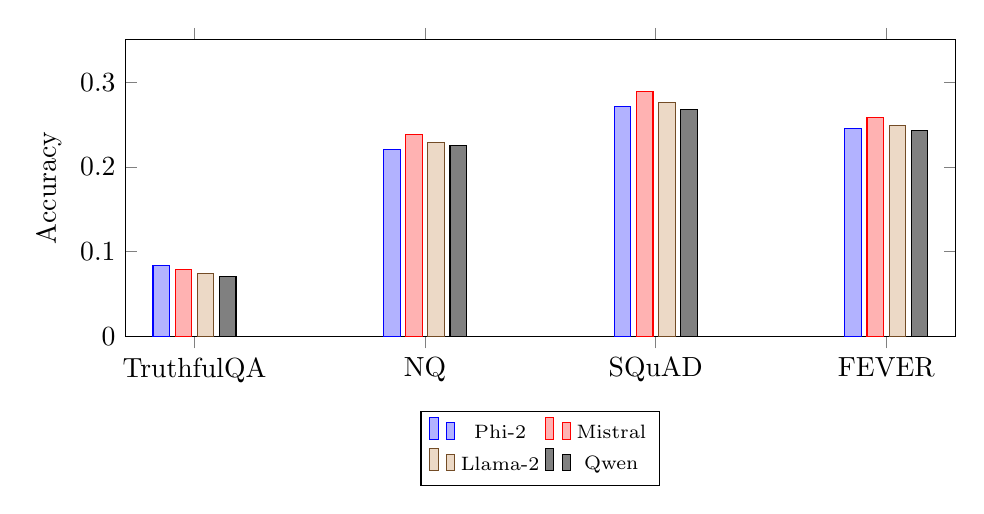
\begin{tikzpicture}
\begin{axis}[
    ybar,
    bar width=6pt,
    width=\linewidth,
    height=5.35cm,
    ylabel={Accuracy},
    symbolic x coords={TruthfulQA,NQ,SQuAD,FEVER},
    xtick=data,
    ymin=0, ymax=0.35,
    legend style={
        at={(0.5,-0.25)},
        anchor=north,
        legend columns=2,
        font=\scriptsize
    }
]
\addplot coordinates {(TruthfulQA,0.084) (NQ,0.221) (SQuAD,0.271) (FEVER,0.245)};
\addplot coordinates {(TruthfulQA,0.079) (NQ,0.238) (SQuAD,0.289) (FEVER,0.258)};
\addplot coordinates {(TruthfulQA,0.074) (NQ,0.229) (SQuAD,0.276) (FEVER,0.249)};
\addplot coordinates {(TruthfulQA,0.071) (NQ,0.225) (SQuAD,0.268) (FEVER,0.243)};
\legend{Phi-2,Mistral,Llama-2,Qwen}
\end{axis}
\end{tikzpicture}
\caption{Accuracy comparison across datasets (zero-shot)}
\label{fig:zs-acc}
\end{figure}

\begin{figure}[H]
\centering
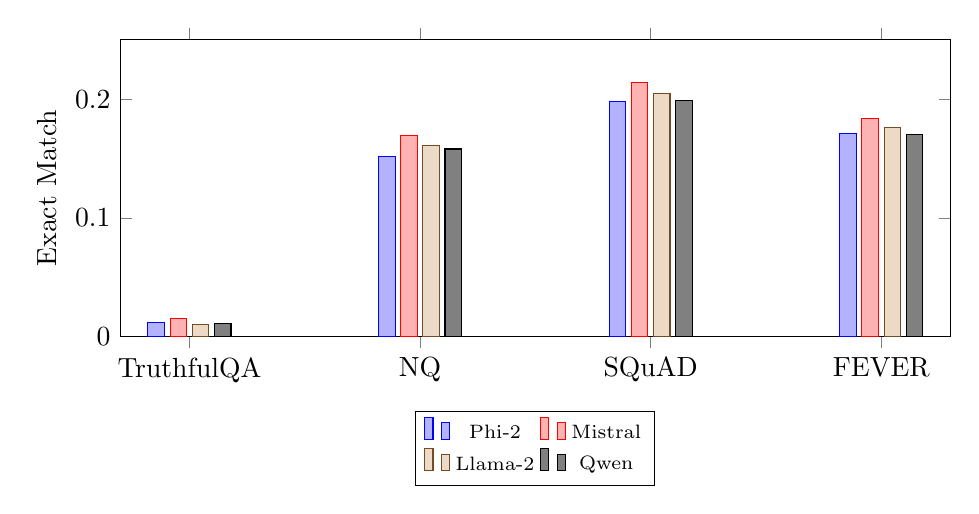
\begin{tikzpicture}
\begin{axis}[
    ybar,
    bar width=6pt,
    width=\linewidth,
    height=5.35cm,
    ylabel={Exact Match},
    symbolic x coords={TruthfulQA,NQ,SQuAD,FEVER},
    xtick=data,
    ymin=0, ymax=0.25,
    legend style={
        at={(0.5,-0.25)},
        anchor=north,
        legend columns=2,
        font=\scriptsize
    }
]
\addplot coordinates {(TruthfulQA,0.012) (NQ,0.152) (SQuAD,0.198) (FEVER,0.171)};
\addplot coordinates {(TruthfulQA,0.015) (NQ,0.169) (SQuAD,0.214) (FEVER,0.184)};
\addplot coordinates {(TruthfulQA,0.010) (NQ,0.161) (SQuAD,0.205) (FEVER,0.176)};
\addplot coordinates {(TruthfulQA,0.011) (NQ,0.158) (SQuAD,0.199) (FEVER,0.170)};
\legend{Phi-2,Mistral,Llama-2,Qwen}
\end{axis}
\end{tikzpicture}
\caption{Exact match comparison across datasets (zero-shot)}
\label{fig:zs-em}
\end{figure}

\begin{figure}[H]
\centering
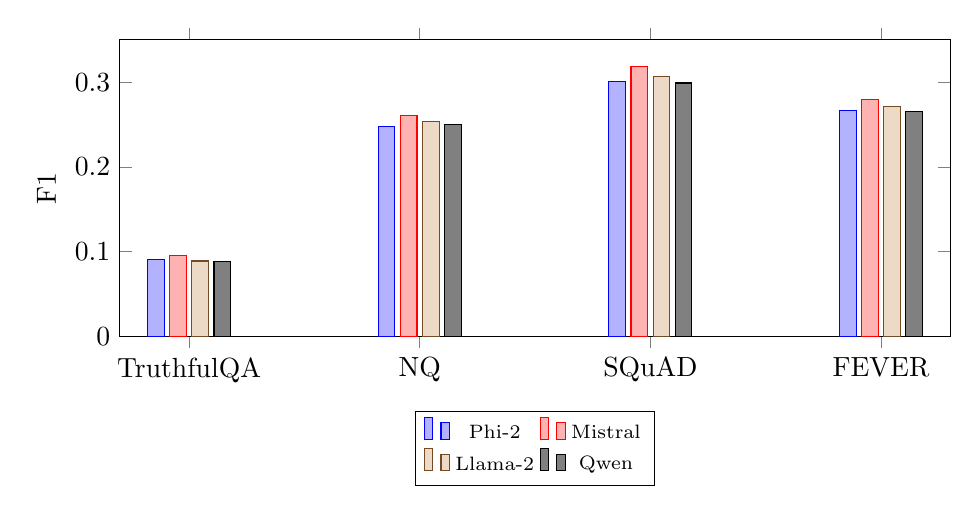
\begin{tikzpicture}
\begin{axis}[
    ybar,
    bar width=6pt,
    width=\linewidth,
    height=5.35cm,
    ylabel={F1},
    symbolic x coords={TruthfulQA,NQ,SQuAD,FEVER},
    xtick=data,
    ymin=0, ymax=0.35,
    legend style={
        at={(0.5,-0.25)},
        anchor=north,
        legend columns=2,
        font=\scriptsize
    }
]
\addplot coordinates {(TruthfulQA,0.091) (NQ,0.248) (SQuAD,0.301) (FEVER,0.267)};
\addplot coordinates {(TruthfulQA,0.095) (NQ,0.261) (SQuAD,0.318) (FEVER,0.279)};
\addplot coordinates {(TruthfulQA,0.089) (NQ,0.254) (SQuAD,0.307) (FEVER,0.271)};
\addplot coordinates {(TruthfulQA,0.088) (NQ,0.250) (SQuAD,0.299) (FEVER,0.265)};
\legend{Phi-2,Mistral,Llama-2,Qwen}
\end{axis}
\end{tikzpicture}
\caption{F1 comparison across datasets (zero-shot)}
\label{fig:zs-f1}
\end{figure}

\begin{figure}[H]
\centering
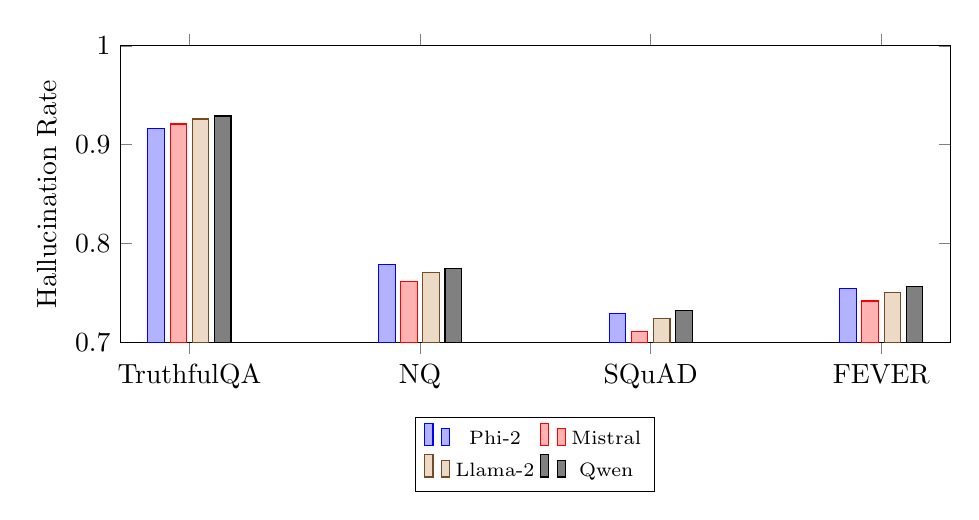
\begin{tikzpicture}
\begin{axis}[
    ybar,
    bar width=6pt,
    width=\linewidth,
    height=5.35cm,
    ylabel={Hallucination Rate},
    symbolic x coords={TruthfulQA,NQ,SQuAD,FEVER},
    xtick=data,
    ymin=0.7, ymax=1,
    legend style={
        at={(0.5,-0.25)},
        anchor=north,
        legend columns=2,
        font=\scriptsize
    }
]
\addplot coordinates {(TruthfulQA,0.916) (NQ,0.779) (SQuAD,0.729) (FEVER,0.755)};
\addplot coordinates {(TruthfulQA,0.921) (NQ,0.762) (SQuAD,0.711) (FEVER,0.742)};
\addplot coordinates {(TruthfulQA,0.926) (NQ,0.771) (SQuAD,0.724) (FEVER,0.751)};
\addplot coordinates {(TruthfulQA,0.929) (NQ,0.775) (SQuAD,0.732) (FEVER,0.757)};
\legend{Phi-2,Mistral,Llama-2,Qwen}
\end{axis}
\end{tikzpicture}
\caption{Hallucination rate comparison across datasets (zero-shot)}
\label{fig:zs-hr}
\end{figure}

\subsection{Few-Shot Results Analysis}
The few-shot results show clear improvements over the zero-shot setting across all models and datasets. Accuracy, EM, and F1 scores increase, especially for structured datasets such as SQuAD and Natural Questions, where models benefit from example-based guidance. Mistral performs best across most metrics, followed by Llama-2 and Qwen, while Phi-2 shows slightly lower performance. Hallucination rates decrease compared to zero-shot, but the improvement is limited. TruthfulQA remains the most difficult dataset, with hallucination rates still above 89\%, indicating that models struggle with misleading or misconception-based questions. In contrast, SQuAD achieves better accuracy and lower hallucination rates than TruthfulQA, though hallucinations remain common overall. Table~\ref{tab:fewshot} summarizes few-shot numbers by dataset and model.

\vspace{0.5\baselineskip}
\begingroup
\centering
\captionsetup{skip=4pt}
\captionof{table}{Few-shot performance across datasets}
\label{tab:fewshot}
\small
\setlength{\tabcolsep}{3.5pt}
\begin{tabular}{l lcccc}
\hline
Dataset & Model & Acc & EM & F1 & HR \\
\hline
TruthfulQA & Phi-2      & 0.102 & 0.018 & 0.118 & 0.898 \\
           & Mistral    & 0.095 & 0.021 & 0.124 & 0.905 \\
           & Llama-2    & 0.091 & 0.017 & 0.119 & 0.909 \\
           & Qwen       & 0.088 & 0.019 & 0.121 & 0.912 \\

NQ         & Phi-2      & 0.249 & 0.178 & 0.276 & 0.751 \\
           & Mistral    & 0.266 & 0.195 & 0.289 & 0.734 \\
           & Llama-2    & 0.258 & 0.187 & 0.282 & 0.742 \\
           & Qwen       & 0.252 & 0.181 & 0.277 & 0.748 \\

SQuAD      & Phi-2      & 0.302 & 0.226 & 0.334 & 0.698 \\
           & Mistral    & 0.321 & 0.241 & 0.352 & 0.679 \\
           & Llama-2    & 0.309 & 0.233 & 0.341 & 0.691 \\
           & Qwen       & 0.301 & 0.225 & 0.332 & 0.699 \\

FEVER      & Phi-2      & 0.279 & 0.198 & 0.301 & 0.721 \\
           & Mistral    & 0.293 & 0.212 & 0.314 & 0.707 \\
           & Llama-2    & 0.284 & 0.205 & 0.307 & 0.716 \\
           & Qwen       & 0.276 & 0.197 & 0.299 & 0.724 \\
\hline
\end{tabular}
\par
\endgroup

\noindent Figure~\ref{fig:fs-acc}--\ref{fig:fs-hr} plot the few-shot metrics from Table~\ref{tab:fewshot}.

\begin{figure}[H]
\centering
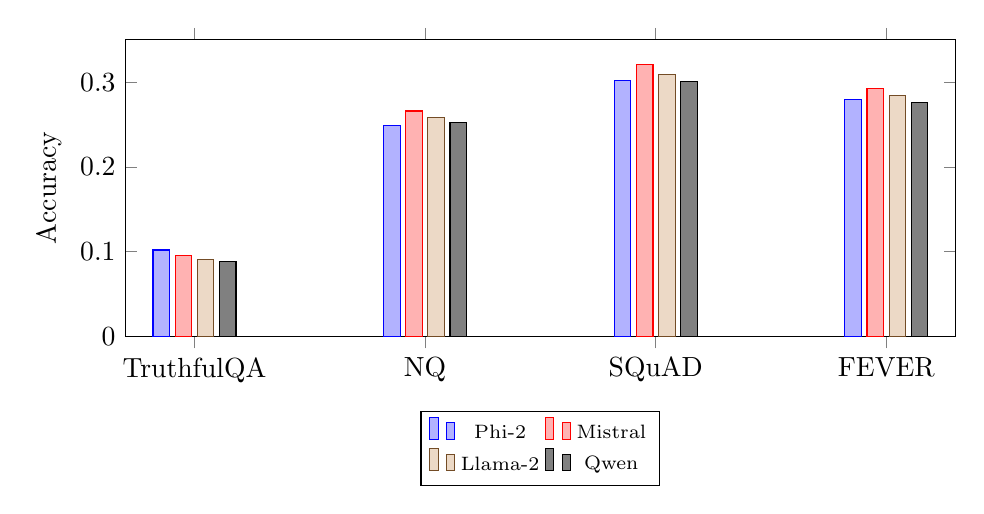
\begin{tikzpicture}
\begin{axis}[
    ybar,
    bar width=6pt,
    width=\linewidth,
    height=5.35cm,
    ylabel={Accuracy},
    symbolic x coords={TruthfulQA,NQ,SQuAD,FEVER},
    xtick=data,
    ymin=0, ymax=0.35,
    legend style={
        at={(0.5,-0.25)},
        anchor=north,
        legend columns=2,
        font=\scriptsize
    }
]
\addplot coordinates {(TruthfulQA,0.102) (NQ,0.249) (SQuAD,0.302) (FEVER,0.279)};
\addplot coordinates {(TruthfulQA,0.095) (NQ,0.266) (SQuAD,0.321) (FEVER,0.293)};
\addplot coordinates {(TruthfulQA,0.091) (NQ,0.258) (SQuAD,0.309) (FEVER,0.284)};
\addplot coordinates {(TruthfulQA,0.088) (NQ,0.252) (SQuAD,0.301) (FEVER,0.276)};
\legend{Phi-2,Mistral,Llama-2,Qwen}
\end{axis}
\end{tikzpicture}
\caption{Accuracy comparison across datasets (few-shot)}
\label{fig:fs-acc}
\end{figure}

\begin{figure}[H]
\centering
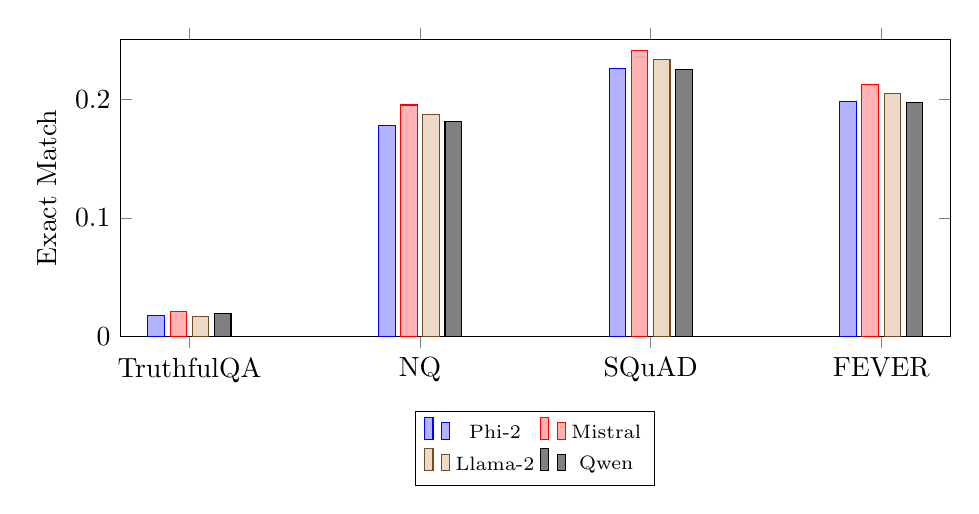
\begin{tikzpicture}
\begin{axis}[
    ybar,
    bar width=6pt,
    width=\linewidth,
    height=5.35cm,
    ylabel={Exact Match},
    symbolic x coords={TruthfulQA,NQ,SQuAD,FEVER},
    xtick=data,
    ymin=0, ymax=0.25,
    legend style={
        at={(0.5,-0.25)},
        anchor=north,
        legend columns=2,
        font=\scriptsize
    }
]
\addplot coordinates {(TruthfulQA,0.018) (NQ,0.178) (SQuAD,0.226) (FEVER,0.198)};
\addplot coordinates {(TruthfulQA,0.021) (NQ,0.195) (SQuAD,0.241) (FEVER,0.212)};
\addplot coordinates {(TruthfulQA,0.017) (NQ,0.187) (SQuAD,0.233) (FEVER,0.205)};
\addplot coordinates {(TruthfulQA,0.019) (NQ,0.181) (SQuAD,0.225) (FEVER,0.197)};
\legend{Phi-2,Mistral,Llama-2,Qwen}
\end{axis}
\end{tikzpicture}
\caption{Exact match comparison across datasets (few-shot)}
\label{fig:fs-em}
\end{figure}

\begin{figure}[H]
\centering
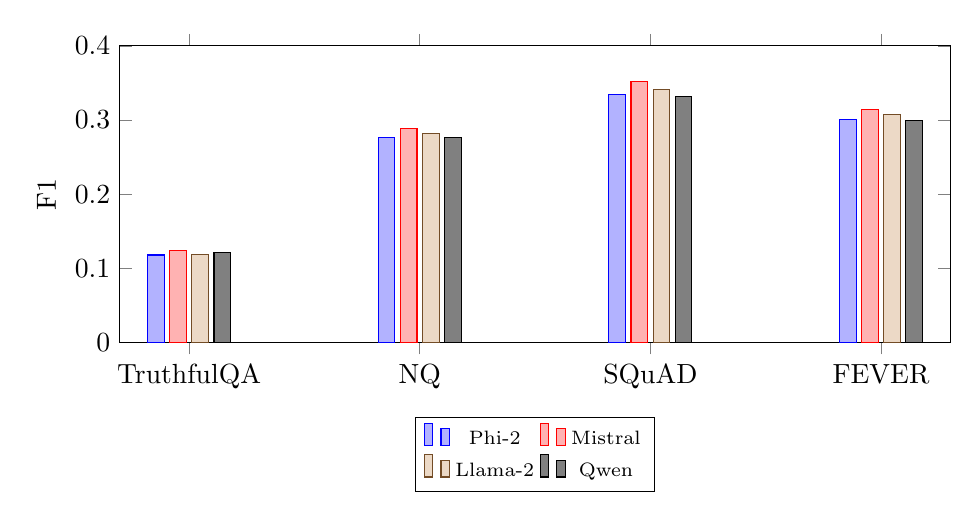
\begin{tikzpicture}
\begin{axis}[
    ybar,
    bar width=6pt,
    width=\linewidth,
    height=5.35cm,
    ylabel={F1},
    symbolic x coords={TruthfulQA,NQ,SQuAD,FEVER},
    xtick=data,
    ymin=0, ymax=0.4,
    legend style={
        at={(0.5,-0.25)},
        anchor=north,
        legend columns=2,
        font=\scriptsize
    }
]
\addplot coordinates {(TruthfulQA,0.118) (NQ,0.276) (SQuAD,0.334) (FEVER,0.301)};
\addplot coordinates {(TruthfulQA,0.124) (NQ,0.289) (SQuAD,0.352) (FEVER,0.314)};
\addplot coordinates {(TruthfulQA,0.119) (NQ,0.282) (SQuAD,0.341) (FEVER,0.307)};
\addplot coordinates {(TruthfulQA,0.121) (NQ,0.277) (SQuAD,0.332) (FEVER,0.299)};
\legend{Phi-2,Mistral,Llama-2,Qwen}
\end{axis}
\end{tikzpicture}
\caption{F1 comparison across datasets (few-shot)}
\label{fig:fs-f1}
\end{figure}

\begin{figure}[H]
\centering
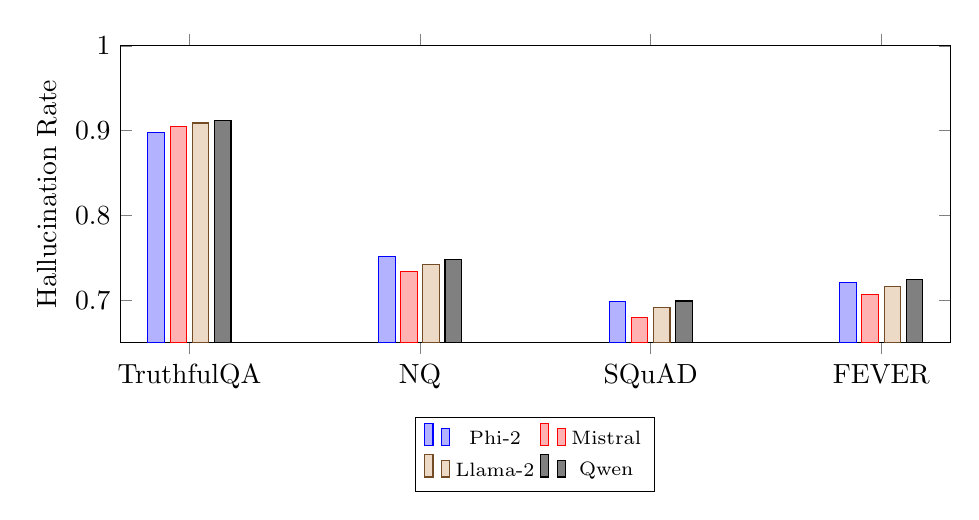
\begin{tikzpicture}
\begin{axis}[
    ybar,
    bar width=6pt,
    width=\linewidth,
    height=5.35cm,
    ylabel={Hallucination Rate},
    symbolic x coords={TruthfulQA,NQ,SQuAD,FEVER},
    xtick=data,
    ymin=0.65, ymax=1,
    legend style={
        at={(0.5,-0.25)},
        anchor=north,
        legend columns=2,
        font=\scriptsize
    }
]
\addplot coordinates {(TruthfulQA,0.898) (NQ,0.751) (SQuAD,0.698) (FEVER,0.721)};
\addplot coordinates {(TruthfulQA,0.905) (NQ,0.734) (SQuAD,0.679) (FEVER,0.707)};
\addplot coordinates {(TruthfulQA,0.909) (NQ,0.742) (SQuAD,0.691) (FEVER,0.716)};
\addplot coordinates {(TruthfulQA,0.912) (NQ,0.748) (SQuAD,0.699) (FEVER,0.724)};
\legend{Phi-2,Mistral,Llama-2,Qwen}
\end{axis}
\end{tikzpicture}
\caption{Hallucination rate comparison across datasets (few-shot)}
\label{fig:fs-hr}
\end{figure}
\endgroup
\FloatBarrier
\raggedbottom

\section{Discussion and Challenges}

The results of this study highlight several important limitations and challenges in evaluating and reducing hallucinations in large language models. One key limitation lies in the evaluation methodology. Metrics such as exact match and containment accuracy rely on surface-level comparison with reference answers, which may incorrectly label semantically correct or partially correct responses as incorrect, leading to an overestimation of hallucination rates. Furthermore, defining hallucination solely based on the absence of reference overlap does not fully capture factual correctness in all cases.

Another practical challenge is computational cost. Evaluating multiple models across several datasets requires substantial GPU resources and time, particularly for larger models.

Answer normalization also affects apparent performance. Models often return full sentences while references are short spans; containment-based accuracy can credit a correct substring, whereas exact match penalizes extra words. Conversely, a fluent but wrong sentence may score well on fluency yet fail every strict metric used here. Readers should therefore interpret high hallucination rate partly as a function of strict matching, not only as a count of ``nonsense'' tokens in isolation.

To address these issues, future work should explore more robust evaluation approaches, including semantic similarity measures and automated fact verification. In addition, integrating retrieval-augmented generation, external knowledge sources, and self-verification mechanisms may help reduce hallucination and improve factual reliability in large language models.


Overall, the experimental results show clear trends across models, datasets, and prompting strategies. First, performance improves consistently when moving from zero-shot to few-shot prompting. Accuracy, exact match, and F1 scores increase across all datasets, while hallucination rates decrease slightly. This indicates that providing examples helps guide the model toward better answers, but the improvement is limited.

Second, dataset difficulty plays an important role. TruthfulQA remains the most challenging dataset, with very low accuracy and very high hallucination rates in both settings. In contrast, SQuAD and Natural Questions show better performance because they are more structured and rely on extractive or well-defined answers. FEVER lies in between, as it requires verification reasoning.

Third, model comparison shows that Mistral performs best overall, followed by Llama-2 and Qwen, while Phi-2 is slightly weaker but still competitive. However, differences between models are relatively small compared to the overall hallucination problem.

Finally, hallucination remains high across all experiments, even in few-shot settings, often above 65–70\%. This shows that current LLMs still struggle with factual reliability, and prompting alone is not enough to fully solve hallucination. More advanced methods are required for improvement.

\section{Concluding Remarks}

This study evaluated the performance of multiple large language models under zero-shot and few-shot settings across four benchmark datasets using accuracy, exact match, F1 score, and hallucination rate as evaluation metrics. The results show that few-shot prompting provides consistent but modest improvements over zero-shot performance, particularly on structured datasets such as SQuAD and Natural Questions. Among the evaluated models, Mistral demonstrates the strongest overall performance, while Phi-2, Llama-2, and Qwen follow with comparable but slightly lower results. Despite these gains, hallucination remains a significant issue across all models and settings, indicating that prompting alone is insufficient to ensure factual reliability. Future work should focus on integrating retrieval-augmented generation, external knowledge grounding, and verification mechanisms to improve factual consistency. Additionally, more robust evaluation strategies that go beyond lexical matching should be explored to better assess model correctness.

\bibliographystyle{ACM-Reference-Format}
\begin{thebibliography}{00}

\bibitem{ji2023survey}
Ziwei Ji et al.
\textit{Survey of hallucination in natural language generation}.
\textit{ACM Computing Surveys}. 2023.

\bibitem{lin2021truthfulqa}
Stephanie Lin et al.
\textit{TruthfulQA: Measuring how models mimic human falsehoods}.
\textit{Proceedings of the 2023 Conference on Empirical Methods in Natural Language Processing (EMNLP)}. 9004--9021.

\bibitem{brown2020language}
Tom B. Brown et al.
\textit{Language models are few-shot learners}.
\textit{Advances in Neural Information Processing Systems (NeurIPS)}. 2020.

\bibitem{lewis2020retrieval}
Patrick Lewis et al.
\textit{Retrieval-augmented generation for knowledge-intensive NLP tasks}.
\textit{Advances in Neural Information Processing Systems (NeurIPS)}. 2020.

\bibitem{touvron2023llama}
Hugo Touvron et al.
\textit{LLaMA: Open and efficient foundation language models}.
\textit{arXiv preprint arXiv:2302.13971}. 2023.

\bibitem{raffel2020exploring}
Colin Raffel et al.
\textit{Exploring the limits of transfer learning with a unified text-to-text transformer}.
\textit{Journal of Machine Learning Research}. 2020.

\bibitem{wei2022chain}
Jason Wei et al.
\textit{Chain-of-thought prompting elicits reasoning in large language models}.
\textit{Advances in Neural Information Processing Systems (NeurIPS)}. 2022.

\bibitem{bubeck2023sparks}
Sébastien Bubeck et al.
\textit{Sparks of artificial general intelligence: Early experiments with GPT-4}.
\textit{arXiv preprint arXiv:2303.12712}. 2023.
\end{thebibliography}

\appendix

\section{Appendix}

\subsection{Experimental Setup}

All experiments were conducted using multiple large language models evaluated under zero-shot and few-shot prompting settings. The same prompts and evaluation procedures were applied consistently across all datasets to ensure fairness. Each model was queried with identical inputs, and outputs were processed using standardized post-processing techniques before evaluation.

\subsection{Datasets}

The evaluation was performed on four benchmark datasets: TruthfulQA, Natural Questions (NQ), SQuAD, and FEVER. These datasets were selected to cover a mix of factual recall, extractive question answering, and fact verification tasks.

\subsection{Metrics}

The following metrics were used for evaluation:
\begin{itemize}
    \item \textbf{Accuracy (Acc):} Measures the proportion of correct predictions.
    \item \textbf{Exact Match (EM):} Measures whether the predicted answer exactly matches the ground truth.
    \item \textbf{F1 Score:} Measures the overlap between predicted and reference answers.
    \item \textbf{Hallucination Rate (HR):} Measures the proportion of incorrect or unsupported responses.
\end{itemize}

\subsection{Implementation Details}

All experiments were implemented in Python using the Hugging Face Transformers and Datasets libraries for model loading, tokenization, and inference. Pre-trained models were accessed directly from the Hugging Face Model Hub without fine-tuning. Inference was performed on a single NVIDIA H100 GPU to handle the computational requirements of running multiple models across datasets. Few-shot prompting was implemented by appending a small number of example demonstrations to each input query.

\subsection{Reproducibility}

To ensure reproducibility, consistent prompts, evaluation scripts, and configurations were used across all experiments. No model-specific tuning was applied, and all runs were executed under identical settings.


\subsection{AI Usage Disclosure}

In the creation of this work, the use of artificial intelligence tools was employed to aid in the debugging of the code, correction of the syntax, and solving any implementation problems. This assignment has been done entirely by myself in terms of designing the experiment, implementing the program, gathering data, and analyzing the results.

\end{document}
